\section{Summary}

\subsection{The Problem}
The Danish Medical Association (DMA) currently has a large amount of courses, online and not, accessible to their members, both free of charge and paid for. The courses’ topics are also widely ranging from informing doctors of new medical treatments to development on their own personal skills. In spite of this, DMA sees very little usage of its available material, especially from the older generation of doctors where their feedback indicates that it is a “break from responsibility” to use the existing continuous education system whilst working. This indicates that time does play a large factor here, since the courses require an allocated time in the doctor’s daily work routine, and sometimes requires entire days being taken out of their schedules to attend courses. Having finished a course, the doctor can add the newly acquired skills to his/her CV but not much more, which also raises the concern of a lack in motivation for taking the courses to begin with. For example, the British Medical Association (BMA) encourages their members to build up their e-portfolio by finishing courses that \fnurl{give credits for their continuous professional development (CPD)}{http://bma.org.uk/developing-your-career/career-progression}, but we have nothing like that in Denmark where each doctor is simply expected to maintain their own continuous education.

The DMA has a lot of data on the usage of their website\footnote{TODO: Add reference to data as an appendix} which show that doctors do visit the learning part of the website, but generally spend very little time there. On average they spend a few minutes, which is far less than the necessary time required to complete a course or in many cases even sign up for one in the first place. Additionally, the traffic to the website mainly comes from desktop computers, but traffic from mobile devices is steadily increasing, although the current learning platform is not optimised for them.

Even though there might be allocated time in doctors’ work schedules, there is not much of an incentive to take courses beyond an obligation to do so, and keeping up with new knowledge might in the end just become a hassle as taking away precious office hours which some doctors think are better spent practicing medicine.

\subsection{In this report}
This report consists of our visions of overall change. In it we propose and suggest innovative changes to DMA’s organization as well as changes to the usage of current available systems in DMA’s domain. We base these changes on the results of the four phases of the MUST method \cite{bodker} i.e the Initiation phase; In-line analysis phase; In-depth analysis phase and finally the Innovation phase. Figure \ref{fig:baseline_plan} shows these four phases and our documented activities within each one.

\begin{figure*}[h!]
 \begin{center}
  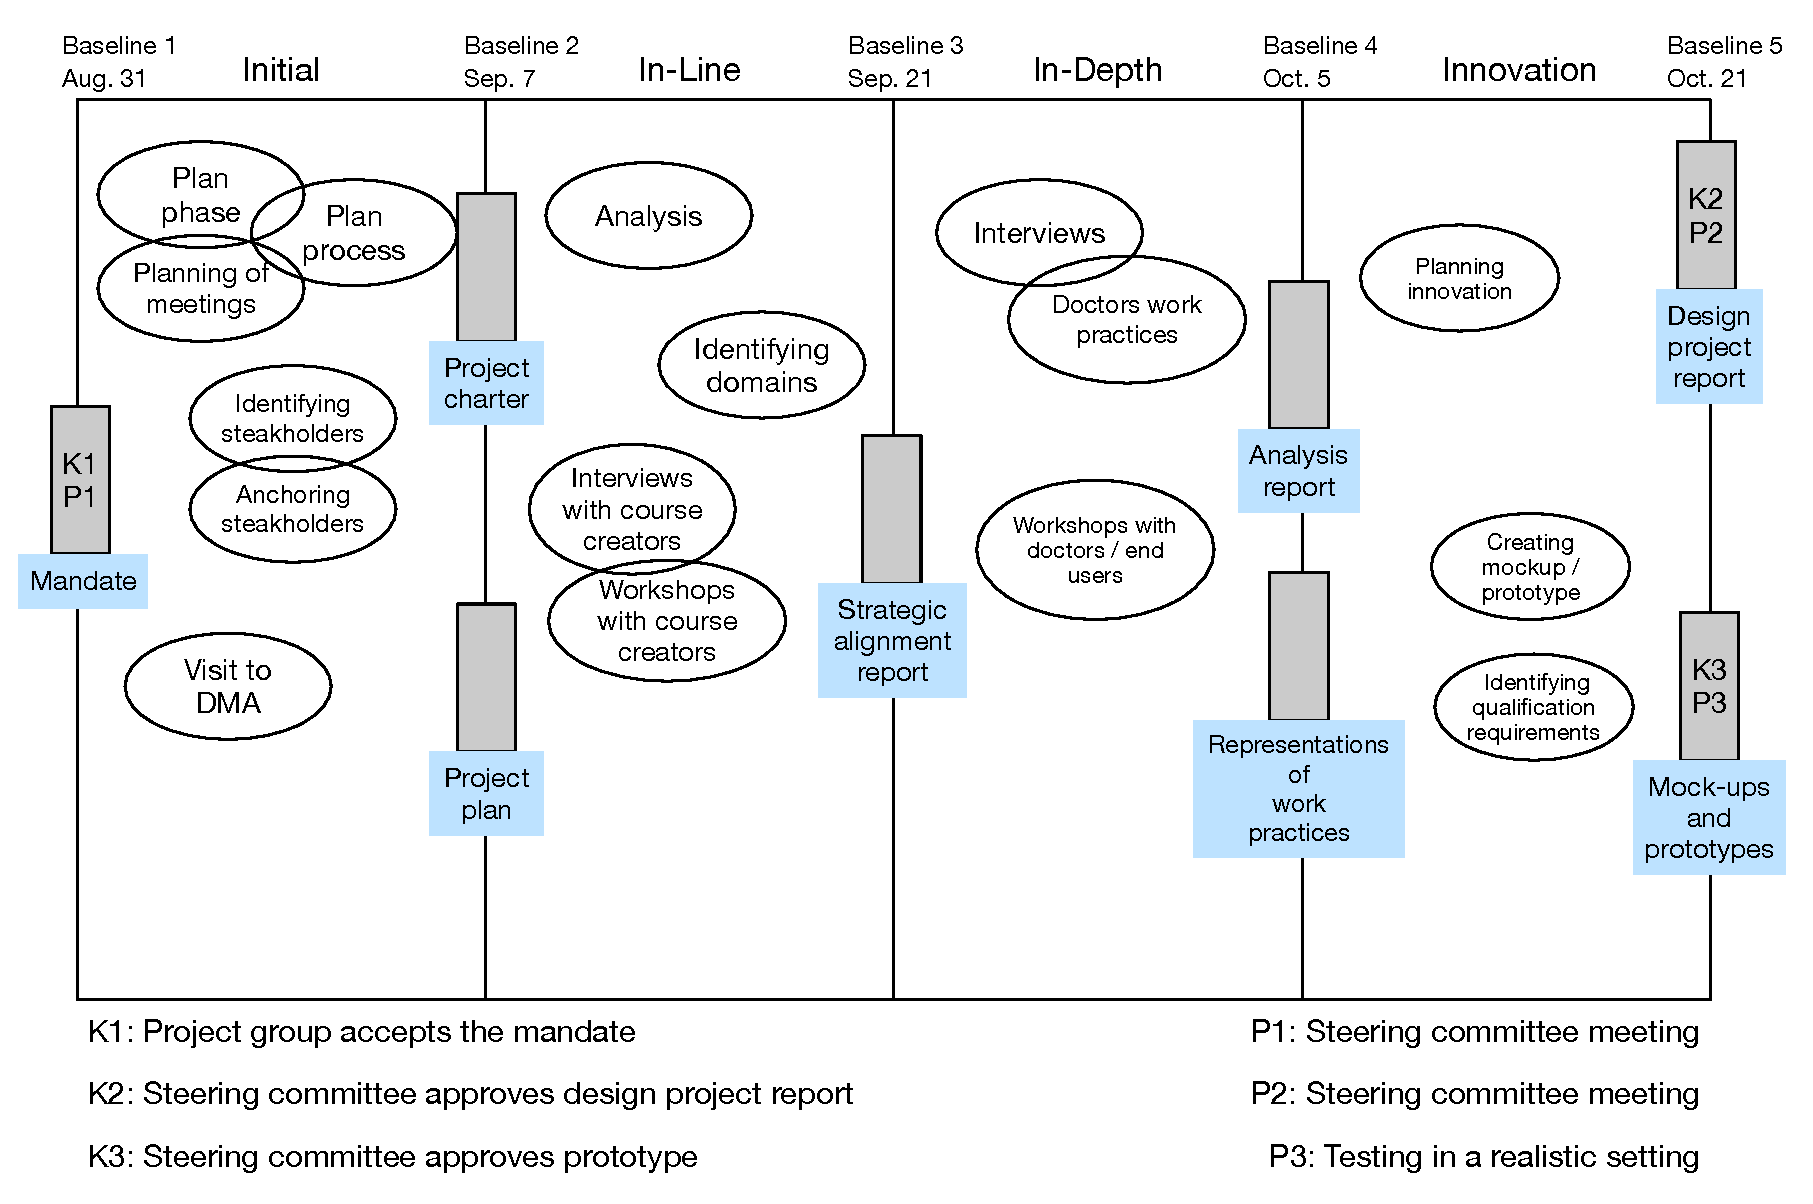
\includegraphics[width=1\textwidth]{figures/baseline-plan.pdf}
  \caption{Our baseline-plan for the project.\label{fig:baseline_plan}}
 \end{center}
\end{figure*}



Given the high complexity of the general problem and our time limitations, we decided to focus the scope of the innovation to something very specific, in this case, the doctors’ time. We have therefore attempted to come up with ideas on how to engage them in a very limited timeframe. This is opposed to coming up with ideas that target completely new platforms for e-learning or making up ideas about how the course material should be presented for doctors (i.e divide courses into multiples of smaller segments).

Our proposed solutions are based on the assumption that doctors are overly busy individuals that have to be engaged with a well defined approach using methods that we like to call Hook and Reel. Hooks can come in different formats, e.g a video, a test or an image, but they all share the same purpose, to hook the doctors and reel them in a very short timeframe.

This report is structured as follows. Section \textit{Methods} on page~\pageref{sec:method}. Section \textit{Objective} on page \pageref{sec:objective} goes through the main points and results of the first three MUST phases. Section \textit{Vision of overall change} on page \pageref{sect:vision} goes into detail of our visions of the overall change, where we identify changes to the technology, DMA’s work organization and required qualifications to implement said changes. Section \textit{Advantages and disadvantages} on page \pageref{sec:advantages} is about the advantages of our proposed solution with regards to DMA’s business strategy. Section \textit{Finances} on page \pageref{sec:finances} talks about the cost of implementation. Section \textit{Implementation strategy and plan} on page \pageref{sec:implementation} introduces our recommended plan to implement our visions of change with regards to technicality and organization. Finally, section \textit{Recommendations and priorities} on page \pageref{sec:recommendations} includes final words on additional recommendations and priorities for DMA.

